\chapter{Flujo de trabajo para la implementación de software para GNC embebido}
\label{ch:especifico2}

Como se pudo observar en el capítulo \ref{ch:especifico1}, se realizó la selección de la tarjeta de desarrollo Zedboard para el desarrollo del proyecto, además de esto uno de los parámetros que se tomó en cuenta fue la compatibilidad de esta con el flujo de trabajo de Yocto Project.

Es por esto que en este capítulo se pretenden establecer los flujos de trabajo para el prototipado de algoritmos de control de orientación y navegación para aplicaciones espaciales. Esto mediante el uso de MATLAB Simulink para tomar un caso de estudio como ejemplo.

Una vez seleccionado el caso de estudio se convierte el código por medio de la transformación de modelo de Simulink a un modelo de código C, esto con el objetivo de poder embeber el código C por medio del flujo de trabajo de Yocto Project y finalmente probar el mismo en la tarjeta de desarrollo seleccionada.

De esta forma se puede comparar los resultados obtenidos y el tiempo de ejecución que llevo la tarea en el computador y en el sistema embebido.


\begin{figure}[h!]
    \centering
    \includegraphics[width=0.3\textwidth]{fig/especifico_2/Diagrama general del proyecto.pdf}
    \caption{Diagrama general del flujo de trabajo propuesto}
    \label{fig:diagrama_flujo_trabajo}
\end{figure}


En la Figura \ref{fig:diagrama_flujo_trabajo}, se muestra un diagrama del flujo de trabajo general. En este capítulo se trabajará en la sección remarcada en rojo la cual engloba la generación del modelo utilizado como caso de estudio, la validación del mismo en MATLAB Simulink, la generación de un código en lenguaje C y la incorporación del mismo en el flujo de trabajo de Yocto Project.

\section{Selección del caso de estudio}

Como caso de estudio se seleccionó una aplicación la cual permitiera una comparación de resultados antes del procesado y después del mismo, es por esto que se decidió implementar un filtro  de tipo paso bajo haciendo uso de los siguientes bloques de MATLAB Simulink. 

\begin{itemize}
    \item Onda seno
    \item Suma
    \item Función de transferencia
    \item Generador de archivo de salida
\end{itemize}

La configuración seleccionada para el primer generador de onda seno es:

\begin{itemize}
    \item Amplitud = 1
    \item Bias = 0 
    \item Frecuencia = 1 rad/s
    \item Fase = 0 
    \item Tiempo de muestreo = 0 
\end{itemize}

Por otro lado, para la segunda onda se tiene la configuración:

\begin{itemize}
    \item Amplitud = 1
    \item Bias = 0 
    \item Frecuencia = 12 rad/s
    \item Fase = 0 
    \item Tiempo de muestreo = 0 
\end{itemize}

Ya que al sumar ondas de diferentes frecuencias, se puede observar un fenómeno llamado modulación, donde la onda resultante presenta un patrón que varía en el tiempo.

\begin{equation}
    y(t) = \sin(t) + \sin(12t)
    \label{eq:funcion_de_suma_de_ondas}
\end{equation}

Por otro lado la función de transferencia a utilizar en el filtro será:

\begin{equation}
    H(S) = \frac{1}{S+1}
    \label{eq:funcion_de_transferencia_filtro}
\end{equation}

Al aplicar el filtro a la señal compuesta,  la onda $\sin(t)$ pasará a través del filtro con poca atenuación, mientras que la onda $\sin(12t)$ será significativamente atenuada debido a su  alta frecuencia.

\begin{figure}[h!]
    \centering
    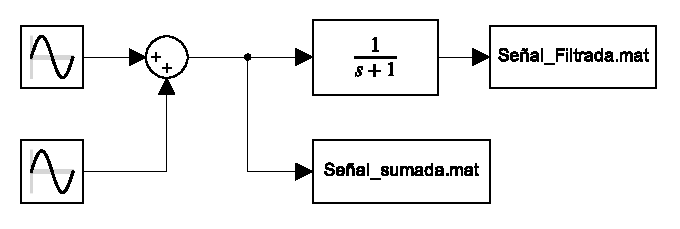
\includegraphics[width=0.5\textwidth]{fig/especifico_2/Diagrama matlab simulink.pdf}
    \caption{Diagrama MATLAB Simulink}
    \label{fig:diagrama_matlab_simulink}
\end{figure}

Estos bloques mencionados anteriormente se colocan como se muestra en la Figura \ref{fig:diagrama_matlab_simulink} de modo que se obtienen como salida del sistema dos archivos, uno llamado señal sumada el cual contiene los datos crudos de la suma de las dos señales y otro denominado señal filtrada el cual contiene los datos de la señal filtrada por la función de transferencia.

\subsection{Simulación del caso de estudio en MATLAB Simulink}\label{subsec:simulacion_caso_de_estudio}

\begin{figure}[h!]
    \centering
    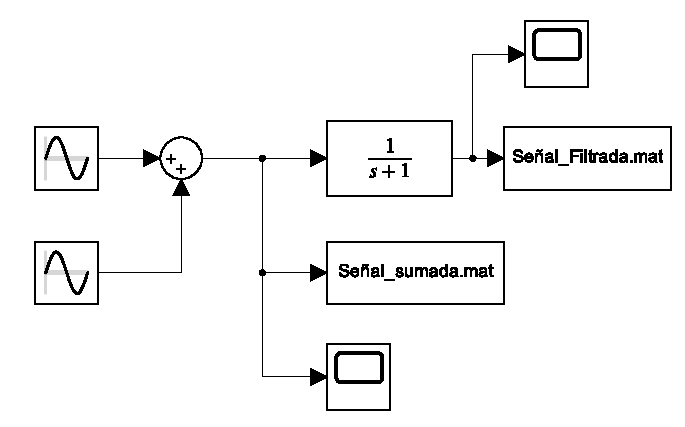
\includegraphics[width=0.5\textwidth]{fig/especifico_2/Diagrama matlab simulink scope.pdf}
    \caption{Diagrama MATLAB Simulink para poder observar las salidas}
    \label{fig:diagrama_matlab_simulink_graficos}
\end{figure}

Utilizando el diagrama de la Figura \ref{fig:diagrama_matlab_simulink}, además de los parámetros configurados anteriormente se colocan dos bloques de gráfico en el diagrama como se muestra en la Figura \ref{fig:diagrama_matlab_simulink_graficos}, esto con el objetivo de poder observar las señales de salida en cada uno de los puntos de interés. 


\begin{figure}[htbp]
    \centering
    \begin{subfigure}[b]{0.45\textwidth}
        \centering
        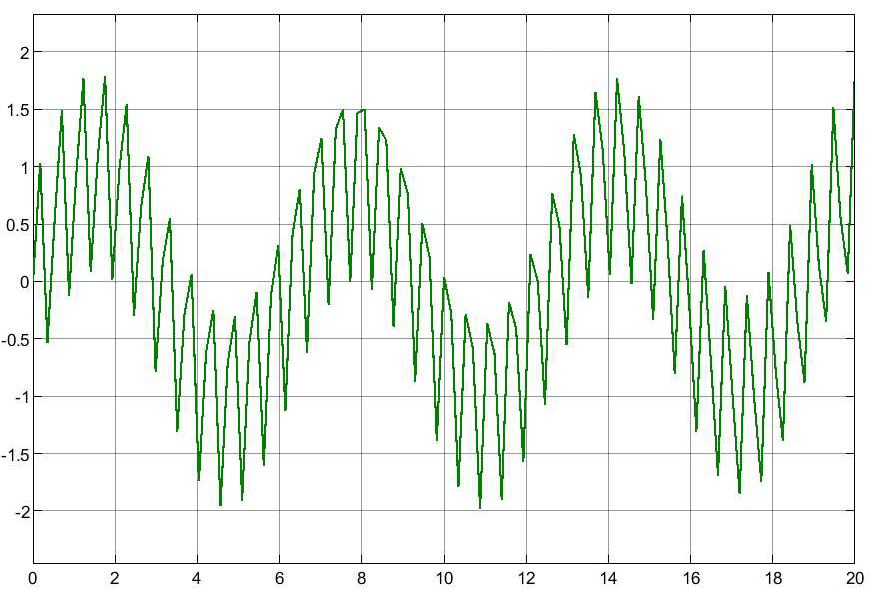
\includegraphics[width=\textwidth]{fig/especifico_2/onda_modulada.pdf}
        \caption{Ondas Moduladas}
        \label{fig:onda_modulada}
    \end{subfigure}
    \hfill
    \begin{subfigure}[b]{0.45\textwidth}
        \centering
        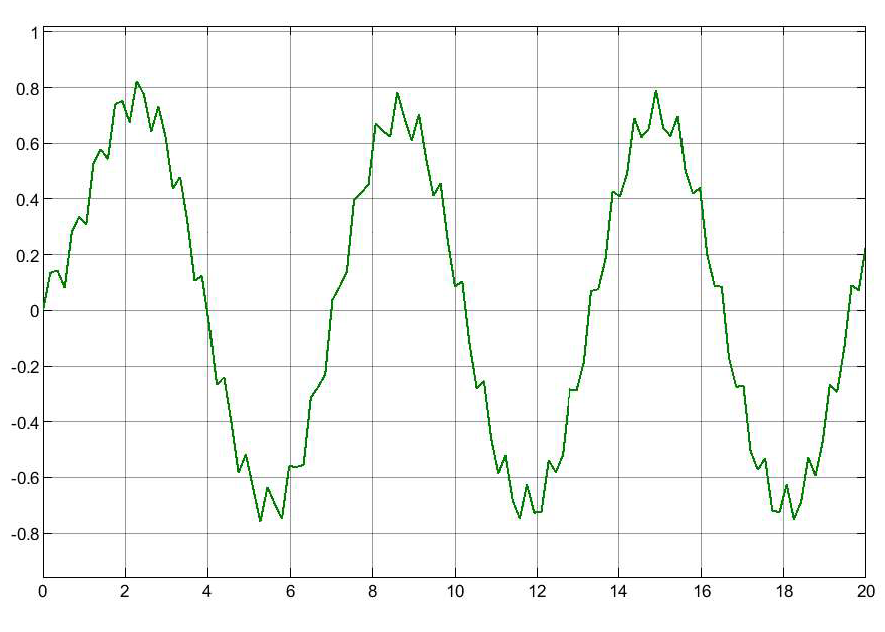
\includegraphics[width=\textwidth]{fig/especifico_2/onda_filtrada.pdf}
        \caption{Onda resultante luego de la función de transferencia}
        \label{fig:onda_filtrada}
    \end{subfigure}
    \caption{Salida resultante del diagrama mostrado en la Figura \ref{fig:diagrama_matlab_simulink_graficos}}
    \label{fig:salida_resultante_diagrama_graficos}
\end{figure}


Como se puede observar en la Figura \ref{fig:onda_modulada} se puede observar la salida de la suma de las dos señales senoidales, por otro lado en la Figura \ref{fig:onda_filtrada} se puede observar la salida de la función de transferencia.

\subsubsection{Resultados obtenidos con la ejecución de la simulación}

Como se mencionó anteriormente los resultados obtenidos se pueden observar en la Figura \ref{fig:salida_resultante_diagrama_graficos}, siendo la salida esperada de la función de transferencia, ya que al ser un filtro paso bajo atenúa las señales que estén por debajo de la frecuencia de corte, que para este filtro es de 1 $rad/s$. Como la señal compuesta contiene una onda seno con frecuencia de 1 $rad/s$ y otra con frecuencia de 12 $rad/s$ es posible observar aun componentes de la frecuencia atenuada.

\section{Flujo de trabajo de la aplicación de transformación de modelo a modelo}

Para poder cumplir con el objetivo de embeber el sistema, se debe de hacer uso del MATLAB Simulink Coder, el cual tiene la capacidad de convertir un sistema de control generado en MATLAB Simulink, en un código C. Algunos de los parámetros que se pueden configurar en este transformador de modelos son: parámetros de la solución, implementación en hardware y generación de código.

A lo largo de este capítulo se definirán los parámetros que se deben de utilizar y el funcionamiento de estos dentro de la generación del código C.

\subsection{Simulink Coder}\label{subsec:simulink_coder}

Una vez comprobado el comportamiento esperado por el caso de estudio se puede proceder con la ejecución del flujo de trabajo de MATLAB Simulink Coder, esto con el fin de transformar el modelo generado en Simulink a un modelo de lenguaje de programación C. Cabe destacar que para esta implementación se utilizó el diagrama que se muestra en la Figura \ref{fig:diagrama_matlab_simulink}, ya que, este solamente contiene como salida los archivos con los datos numéricos del sistema y no contiene las salidas gráficas agregadas en \ref{subsec:simulacion_caso_de_estudio}.


\subsection{Definición de parámetros}

\begin{figure}[h!]
    \centering
    \includegraphics[width=0.8\textwidth]{fig/especifico_2/paso_a_paso_mtmt/apps.png}
    \caption{Pestaña Aplicaciones}
    \label{fig:pestana_apps}
\end{figure}

\begin{figure}[h!]
    \centering
    \includegraphics[width=0.8\textwidth]{fig/especifico_2/paso_a_paso_mtmt/c_code.png}
    \caption{Pestaña código C}
    \label{fig:pestana_c_code}
\end{figure}

\begin{figure}[h!]
    \centering
    \includegraphics[width=0.8\textwidth]{fig/especifico_2/paso_a_paso_mtmt/configuration_parameters.png}
    \caption{Configuración de parámetros}
    \label{fig:pestana_config}
\end{figure}

Para la definición de parámetros, se debe de estar en el entorno de MATLAB Simulink, una vez en el entorno mencionado anteriormente se debe ir a la pestaña denominada Aplicaciones, o bien APPS como se muestra en la Figura \ref{fig:pestana_apps}, se deberá de seleccionar la aplicación denominada Simulink Coder, cuando seleccionamos esta opción se abrirá una pestaña llamada código C, o bien C CODE como se pudo observar en la Figura \ref{fig:pestana_c_code}.

Una vez estemos en la pestaña de código C, debemos de ir a la opción de configuración de parámetros, en la Figura \ref{fig:pestana_c_code} se observa esta opción bajo el nombre de settings, una vez presionada la opción se abre una ventana emergente como la que se muestra en la Figura \ref{fig:pestana_config}, en la pestaña denominada Solver se deberán de proporcionar los datos sobre el tiempo de ejecución de la prueba.

\subsubsection{Selección del procesador objetivo}

\begin{figure}[h!]
    \centering
    \includegraphics[width=0.8\textwidth]{fig/especifico_2/paso_a_paso_mtmt/configuration_parameters_processor.png}
    \caption{Selección del procesador y la familia del procesador}
    \label{fig:pestana_config_procesador}
\end{figure}

Continuando en la sección de configuración de parámetros ahora debemos de ir a la pestaña llamada implementación de hardware o bien Hardware Implementation, en donde deberemos de colocar los datos de Device Vendor el cual hace referencia al tipo de procesador que contiene la tarjeta de desarrollo, para nuestro caso sería ARM Compatible y el Device Type que seria a la familia que pertenece el procesador, para nuestro caso sería un ARM Cortex-A de 32-bits tal y como se muestra en la Figura \ref{fig:pestana_config_procesador}.


\subsubsection{Selección del tipo de archivo de construcción}

Anteriormente configuramos los parámetros de tiempo de operación y procesador de la tarjeta de desarrollo, ahora debemos de configurar el tipo de archivo que se utilizara para la generación de los archivos binarios, como se deberá de realizar una compilación cruzada se debe de elegir un tipo de archivo el cual nos permita compilar los binarios para la ejecución del sistema sin importar el sistema operativo de la máquina host. Es por esto que se debe de seleccionar en la pestaña de Code Generation el Toolchain denominado CMake tal y como se muestra en la Figura \ref{fig:pestana_config_output_file}, además de esto se debe de marcar tanto la opción denominada como Generate code only, como Package code and artifacts, esta última nos genera como salida un archivo comprimido con todos los requerimientos de la aplicación para poder ser construida.


\begin{figure}[h!]
    \centering
    \includegraphics[width=0.8\textwidth]{fig/especifico_2/paso_a_paso_mtmt/configuration_output_file.png}
    \caption{Selección del tipo de archivo de construcción}
    \label{fig:pestana_config_output_file}
\end{figure}

\subsubsection{Generación de archivos de compilación}

Una vez configurados todos los parámetros mencionados anteriormente debemos de proceder con la construcción de los archivos, para esto se debe de ir a la barra de tareas a la opción denominada como generar código, la misma se puede observar en la Figura \ref{fig:pestana_c_code} bajo el nombre de Build.

\subsection{Contenedor para compilación de los binarios}

Para poder generar la compilación cruzada es necesario crear un contenedor para poder utilizar Ubuntu 20.04, ya que esta versión es la que presenta mayor compatibilidad con las dependencias contenidas en el flujo de trabajo de Yocto Project que se utiliza. 


\begin{lstlisting}[language=bash, caption={Comando para la instalacion de docker}, label=lst:install_docker]
    sudo apt install docker.io
\end{lstlisting}

\begin{lstlisting}[language=bash, caption={Comando para la instalacion de Ubuntu 20.04}, label=lst:install_20_04_ubuntu]
    sudo docker run -it ubuntu:20.04 /bin/bash
\end{lstlisting}

Para poder generar este contenedor primeramente se debe de satisfacer la dependencia de tener instalado docker.io, esto se logra por medio del comando que se muestra en \ref{lst:install_docker},seguido de esto, se puede hacer uso del comando \ref{lst:install_20_04_ubuntu} el cual se encarga de construir la máquina dentro del entorno del contenedor. Este último comando se encarga de descargar la imagen de Ubuntu 20.04, crea y ejecuta un contenedor en modo interactivo además de proporcionar acceso al terminal del contenedor, donde puedes ejecutar comandos como si fuera una máquina virtual con Ubuntu 20.04.

\subsubsection{Instalación de programas en el contenedor}

\begin{lstlisting}[language=bash, caption={Comando para la instalacion del compilador cruzado}, label=lst:cross_compiler]
    sudo apt install gcc-arm-linux-gnueabihf
\end{lstlisting}

\begin{lstlisting}[language=bash, caption={Comando para la instalacion de CMake}, label=lst:cmake]
    sudo apt install cmake
\end{lstlisting}

\begin{lstlisting}[language=bash, caption={Comando para la instalacion de build essential}, label=lst:build_essential]
    sudo apt install build-essential
\end{lstlisting}

Una vez generado el contenedor debemos de instalar en el mismo el compilador cruzado que para nuestros efectos será arm-linux-gnueabihf-gcc, esto lo podemos hacer mediante el comando que se muestra en \ref{lst:cross_compiler},  CMake el cual es una herramienta de construcción multiplataforma y de código abierto que se utiliza para gestionar la construcción de software utilizando un enfoque basado en proyectos y finalmente build-essential las cuales son herramientas que nos ayudaran a compilar el programa generado en \ref{subsec:simulink_coder} para la arquitectura del procesador.

\begin{figure}[h!]
    \centering
    \includegraphics[width=0.8\textwidth]{fig/especifico_2/paso_a_paso_mtmt/root_folder.png}
    \caption{Archivo comprimido en el directorio swap\_area}
    \label{fig:pestana_swap_area}
\end{figure}

\begin{lstlisting}[language=bash, caption={Comando para la copiar archivos al contenedor}, label=lst:copy_to_container]
    sudo docker cp /direccion/del/archivo 
    <id_de_contenedor>:/direccion/del/contenedor
\end{lstlisting}

\begin{lstlisting}[language=bash, caption={Comando para la copiar archivos del contenedor}, label=lst:copy_from_container]
    sudo docker cp <id_de_contenedor>:/direccion/del/contenedor
    /direccion/del/archivo
\end{lstlisting}

Seguido de esto se debe de copiar el archivo comprimido generado en \ref{subsec:simulink_coder}, al contenedor con Ubuntu. Primeramente colocaremos el archivo comprimido en un directorio llamado swap\_area, tal y como se muestra en \ref{fig:pestana_swap_area}. Seguido de esto se debe de descomprimir el archivo. Una vez descomprimido el archivo, como se mencionó anteriormente, lo enviaremos al contenedor haciendo uso del comando \ref{lst:copy_to_container}.

\subsection{Compilación de los binarios}\label{subsec:compilacion_binario}

\begin{lstlisting}[language=bash, caption={Comando para la compilacion del programa}, label=lst:build_cmake_file]
    cmake -DCMAKE_C_COMPILER=arm-linux-gnueabihf-gcc 
    CMakeLists.txt -DMATLAB_ROOT=/home/test/simple_filter/R2024b/
\end{lstlisting}

\begin{figure}[h!]
    \centering
    \includegraphics[width=0.8\textwidth]{fig/especifico_2/paso_a_paso_mtmt/cmake_file.png}
    \caption{Make File}
    \label{fig:make_file}
\end{figure}


\begin{figure}[h!]
    \centering
    \includegraphics[width=0.8\textwidth]{fig/especifico_2/paso_a_paso_mtmt/binario_compilado.png}
    \caption{Binario llamado simple\_filter}
    \label{fig:binario_compilado}
\end{figure}

Para la compilación del archivo binario se deberá hace uso del comando \ref{lst:build_cmake_file} por el cual se construirá el Makefile, tal y como se muestra en la Figura \ref{fig:make_file}, una vez generado el Makefile se ejecutó el comando make el cual da como salida los binarios requeridos para la ejecución del programa. Los mismos se observan como se muestra en la Figura \ref{fig:binario_compilado}.

Una vez compilado el archivo binario, se puede continuar con el flujo que se presenta en el diagrama que se muestra en la Figura \ref{fig:diagrama_flujo_trabajo}, lo cual sería la implementación de los binarios en una imagen de yocto.


\section{Flujo de Trabajo Herramienta desarrollada por mi persona}

Como se pudo observar anteriormente se realizó la compilación cruzada de un caso de estudio, el mismo ahora se debe de implementar en un sistema operativo a la medida mediante el flujo de trabajo de Yocto Project, como se mencionó en \ref{subsec:yocto}, Yocto Project es un marco de trabajo utilizado para el desarrollo de sistemas embebidos especializado en la construcción de distribuciones de Linux a la medida. 

\begin{figure}[h!]
    \centering
    \includegraphics[width=0.8\textwidth]{fig/especifico_2/Flujo de trabajo de mi idea.pdf}
    \caption{Flujo de trabajo Yocto}
    \label{fig:flujo_yocto}
\end{figure}

En el desarrollo de esta seccion se muestran los pasos que se siguieron para la generación de una imagen mínima, la integración de una capa personalizada con el binario generado en \ref{subsec:compilacion_binario} y la implementación de la misma en la tarjeta de desarrollo seleccionada.

\subsection{Sistema operativo para desarrollo}

Como sistema operativo de desarrollo se utilizó Ubuntu 22.04 LTS, en una computadora con las siguientes características:

\begin{itemize}
    \item Procesador - Intel Corei9-13980HX 
    \item Almecenamiento - 500 GB
    \item Memoria RAM - 16 GB 
\end{itemize}

\subsection{Generación de un contenedor}

Para el desarrollo del marco de trabajo de Yocto se decidió implementar un contenedor, esto debido a que la versión de Yocto para la cual se encontraba un paquete de soporte para la tarjeta de desarrollo es Yocto Zeus 3.0, este fue liberado en octubre del 2019, por tanto no era soportado por la versión de Linux del computador de desarrollo, es por esto que se tomó la decisión de utilizar un contenedor el cual ejecutara la versión de Ubuntu 16.04 LTS. 

\begin{lstlisting}[language=bash, caption={Comando para la instalacion de Ubuntu 16.04}, label=lst:install_16_04_ubuntu]
    sudo docker run -it ubuntu:16.04 /bin/bash
\end{lstlisting}

Para la generación del contenedor se hace uso del comando que se muestra en \ref{lst:install_16_04_ubuntu}, el cual se encarga de darnos un contenedor con Ubuntu 16.04 LTS.Ademas de esto debemos de instalar algunos requerimientos como lo son:

\begin{itemize}
    \item tree : para poder visualizar árboles de dependencia
    \item vim : para poder editar archivos de texto
    \item etc \dots
\end{itemize}

\subsubsection{Creación de un usuario no root}

Para el uso del marco de trabajo de Yocto se debe de generar un usuario no root, esto principalmente por razones de seguridad y manejo adecuado de permisos. El usuario se puede generar por medio de los siguientes comandos:

\begin{lstlisting}[language=bash, caption={Generacion de usuario no root}, label=lst:no_root_user]
    apt - get install -y sudo
    useradd - ms/bin/bash myuser
    echo "myuser:password" | chpasswd
    usermod - aG sudo myuser
\end{lstlisting}

De forma que según el comando observado en \ref{lst:no_root_user}, en la primera línea instalamos sudo, seguido de esto en la segunda línea se agrega el usuario denominado "myuser", en la tercera línea se genera una contraseña para este usuario la cual se define como "chpasswd", finalmente se agrega en el archivo usermod el nuevo usuario. 

\begin{lstlisting}[language=bash, caption={Iniciar usuario no root}, label=lst:no_root_user_log]
    su - myuser
\end{lstlisting}


Cada vez que iniciemos el contenedor siempre lo haremos como usuario root, para poder iniciar con el usuario no root llamado "myuser" se debe de hacer uso del comando que se muestra en \ref{lst:no_root_user_log}.

\subsection{Yocto Project}

Como se observó en \ref{subsec:yocto}, yocto presenta flexibilidades a la hora de configurar un sistema permitiendo al desarrollador seleccionar paquetes específicos y personalizar el sistema operativo.

\begin{lstlisting}[language=bash, caption={Requerimientos Yocto Zeus}, label=lst:yocto_requirements]
    sudo apt - get install gawk wget git - core diffstat unzip texinfo
    gcc - multilib build - essential chrpath socat cpio python python3
    python3 - pip python3 - pexpect xz - utils debianutils 
    iputils - ping python3 - git python3 - jinja2 
    libegl1 - mesa libsdl1 .2 - dev pylint3 xterm
\end{lstlisting}

Para que el mismo funcione de forma correcta debemos de instalar los requerimientos del marco de trabajo los cuales se pueden observar en \ref{lst:yocto_requirements}.

\begin{lstlisting}[language=bash, caption={Version de Yocto}, label=lst:yocto_clone]
    git clone -b zeus https://git.yoctoproject.org/git/poky
    cd poky
\end{lstlisting}

\begin{lstlisting}[language=bash, caption={BSP para Zedboard}, label=lst:yocto_zedboard]
    git clone -b zeus https://github.com/Xilinx/meta-xilinx
    git clone -b zeus https://github.com/openembedded/meta-openembedded.git
\end{lstlisting}

La versión de yocto a utilizar se debe de clonar de \ref{lst:yocto_clone}, seguido de esto se debe de ir a la rama de la versión Yocto Zeus. Además de clonar este repositorio se debe de ingresar al directorio denominado poky y clonar dentro del repositorio \ref{yocto_zedboard} el cual contiene en su rama llamada Zeus la versión de paquete de soporte para la tarjeta requerida para generar una imagen para la tarjeta de desarrollo seleccionada.

\begin{lstlisting}[language=bash, caption={Configuraciones adicionales}, label=lst:aditional_config]
    source oe - init - build - env
    
    echo "MACHINE ??=\"zedboard-zynq7\"" >> conf/local.conf
    echo "IMAGE_FEATURES +=\"package-management\"" >> conf/local.conf
    echo "DISTRO_HOSTNAME =\"zynq\"" >> conf/local.conf
    
    bitbake-layers add-layer ../meta-xilinx/meta-xilinx-bsp/
    bitbake-layers add-layer ../meta-openembedded/meta-oe/
\end{lstlisting}

Algunas configuraciones adicionales que se deben de realizar se muestran en \ref{lst:aditional_config}.

\subsection{Creacion de una capa de yocto}

Para la generacion de una capa de yocto primero se debe de inicializar el entorno de desarrollo esto mediante el comando que se muestra en \ref{}, este se encarga de generar todos los archivos necesarios para poder hacer uso de las variables de entorno con las cuales opera el marco de trabajo de Yocto, seguido de esto se debe de utilzair el siguiente comando el cual se encargara de generar el arbol de directorios que se puede observar en la Figura \ref{}. Una vez implementado este comando se debe de hacer uso de este comando para poder agregar la capa al archivo denominado xxxx el cual contiene todas las rutas de acceso a las capas requeridas para generar la imagen.

\subsection{Caso de estudio}

En esta seccion se integrara el caso de estudio generado en \ref{}, a un sistema operativo a la medida por medio de el marco de trabajo de Yocto Project, primeramente se generara una capa personalizada, seguido de esto se generara el archivo de instalacion con el cual la capa personalizada pasara a ser parte del sistema de archivos del sistema embebido, tambien se generara la imagen minima la cual consiste en un sistema de arranque y el sistema de archivos y finalmente se implementaran estos en la tarjeta de desarrollo seleccionada en \ref{}.

\subsection{Integración del programa generado a la capa de Yocto}

Para la implementacion de la los binarios generados en \ref{}, se deben de generar algunos directarios, esto con el objetivo de mantener un entorno limpio y ordenado, para contener todos los directorios se genera un directorio llamado xxxx el cual dentro del mismo debera de contener un directorio llamado xxx el cual se encargara de contener el archivo de configuracion de la capa llamado xxxx el cual se genera mediante el comando que se observa en \ref{}, ademas de geenerar este archivo se debe de crear un directorio llamado xxxx que sera el encargado de contener los binarios compilados en \ref{}.

\subsubsection{.bb}

Como se mencionó anteriormente el archivo llamado xxxx.bb es el encargado de la configuracion de la capa, el mismo contiene los comandos de instalacion y la direccion en donde se encontraran los binarios en el sistema de archivos de la imagen del sistema embebido.

La estructura que debe de contener ese archivo para instalar binarios en el sistema son las que se puden observar en \ref{}.

\subsection{Generacion de la imagen minima}

Antes de generar la imagen minima se debe de tener en consideracion ejecutar la linea de comando que se muestra en \ref{}, esto con el fin de generar archivos de xxxx en lugar de xxxx. Una vez generados estos cambios se debe de iniciar de nuevo el entorno por medio del comando \ref{}, seguido de esto se debera de ejecutar el comando de xxx el cual se encarga de comenzar a generar la imagen minima. 

\subsection{Implementacion de la imagen minima en la tarjeta de desarrollo zedboard}

Para la implementacion de la imagen minima en la tarjeta de desarrollo de deben de seguir los siguientes pasos en la maquina Host:

\begin{enumerate}
    \item Se debe de formatear la tarjeta SD de al menos 4 GB, las pariticiones de la misma se tienen que observar de la siguiente forma 
    \begin{itemize}
        \item root = 100 MB FAT 32
        \item File System = 3.5 GB ext6(linux filesystem format)
        \end{itemize} 
    \item Seguido de esto se debe de ir a la ruta xxx/xxxx/xxxx/xxxx/xxxx y se deben de copiar los archivos de el contenedor a la maquina host mediante el comando que se muestra en \ref{}, esto con el objetivo de poder enviar los archivos a la tarjeta SD
\end{enumerate}

Para el sistema Root se deberan de copiar los archivos mediante el comando que se muestra en \ref{}, por otro lado en la particion denominada xxxx se debe de copiar el archvivo xxxx mediante el uso del comando xxxxx el cual se muestra en \ref{}.

\subsection{Conexion de la tarjeta de desarrollo con el computador host}

Como protocolo de comunicacion se establece de primera mano UART , el cual como se menciono en \ref{} consiste en xxxxxxxx y en el caso de la tarjeta de desarrollo se conecta segun s emeustra en el diagrama de la Figura xxxxx, para poder leer la consola se hace uso de Minicom el cual se encarga de xxxxxxxxxxxxxxx.

(Imagen del diagrama de conexion de la tarjeta y el computador por medio de UART)

Seguido de esto se establecio la conexion por medio de SSH el cual como se menciona en \ref{}, consiste en xxxxxxxxx ademas de xxxxxx. 

El diagrama de este protocolo de comunicacion se puede observar en \ref{}.


\subsection{Ejecución del caso de estudio y resultados}

Una vez implementada la imagen de Yocto en la tarjeta de desarrollo se puede ejecutar el caso de estudio por medio de xxxxxx, ademas de esto los resultados se pueden transmitir al computador por medio del comando xxxxxx, seguido de esto, haciendo uso de un codigo generado en python se pueden obtener los graficos de las sennales obtenidas mediante la ejecucion del binario contenido en la imagen minima.

(imagen que contenga los dos graficos, a la inquizarda el de las dos senales sumadas y a la derecha el de la senal filtrada)

\subsection{Comparacion de resultados}

Como se pudo observar, con la comparacion realizada, obtenemos que los datos tiene una desviacion de xxxxx ademas de xxxxxx, es por esto que podemos determinar que la implementacion de sistemas de control es viable segun lo demuestra el caso de estudio.


\section{Reflexion final}